\documentclass[a4paper,14pt]{extarticle}

\usepackage[a4paper,top=20mm,right=20mm,bottom=20mm,left=30mm]{geometry}
\usepackage[T1,T2A]{fontenc}
\usepackage[utf8]{inputenc}
\usepackage[russian]{babel}
\usepackage{indentfirst}
\usepackage{titlesec}
\usepackage{graphicx}
\usepackage{listings}

\renewcommand{\baselinestretch}{1.3}
\titleformat{\section}{\normalsize\bfseries}{\thesection}{1em}{}
\titleformat{\subsection}{\normalsize}{\thesection}{1em}{}
\setlength{\parindent}{12.5mm}

\begin{document}

  \newpage\thispagestyle{empty}
  \begin{center}
    \textbf{
      \MakeUppercase{
        Министерство науки и высшего образования Российской Федерации\\
        Федеральное государственное бюджетное образовательное учреждение высшего образования\\
        <<Вятский Государственный Университет>>\\
      }
      Институт математики и информационных систем\\
      Факультет автоматики и вычислительной техники\\
      Кафедра электронных вычислительных машин
    }
  \end{center}
  \vfill

  \begin{center}
    Отчет по лабораторной работе №1\\
    по дисциплине\\
    <<Программирование>>\\
  \end{center}
  \vfill

  \noindent
  \begin{tabular}{ll}
    Выполнил студент гр. ИВТб-1301-05-00 \hspace{8mm} &
    \rule[-1mm]{20mm}{0.10mm}\,/Макаров С.А./\\

    Руководитель зав. кафедры ЭВМ & \rule[-1mm]{20mm}{0.10mm}\,/Долженкова М.Л./\\
  \end{tabular}

  \vfill
  \begin{center}
    Киров 2024
  \end{center}

  \newpage
  \section*{Цель}
  Цель лабораторной работы: закрепить на практике знания о программировании, используя переменные, арифметические операции, условные конструкции, циклы.

  \section*{Задание}
  \begin{enumerate}
    \item Среди введенных N чисел определить длину максимальной возрастающей последовательности.
    
    \item Для заданных натуральных чисел M и N. Получить сумму M младших цифр числа N.
    
    \item Будем называть трехзначное число "красивым", если полусумма его минимальной и максимальной цифры меньше оставшейся. Определите является ли введенное число "красивым".
    
    \item Среди произвольного количества целых чисел определить минимальный порядковый номер наименьшего из них.
    
    \item В некоторой стене осталось не закрытым прямоугольное отверстие размером A на B. Определить, проходит ли кирпич с размерами x, y, z через это отверстие.
    
    \item Заданы координаты вершин прямоугольника со сторонами, параллельными осям координат (x1,y1) и (x2,y2). Определить площадь части прямоугольника, расположенной в первой координатной четверти.
    
    \item Дана не пустая последовательность ненулевых целых чисел. Определить, сколько раз в этой последовательности меняется знак.
    
    \item Необходимо протестировать группу из N человек. Каждый из них вводит: 1 – если он изучал английский язык, 2 – если немецкий, 3 – если французский, 0 – если не изучал никакой. Определите, сколько человек в каждой языковой группе.
    
    \item В катушке с автобусными билетами (номер билета шестизначный) меньший номер билета n, больший m. Определить количество счастливых билетов.
    
    \item В университете на потоке учатся M групп. Каждый месяц декан проводит конкурс на "хорошую" группу. Для этого оценивается число пропущенных занятий каждым студентом группы. и рассчитывается среднее значение по группе Nm, где m номер группы. Если минимальное число пропусков N1, N2, N3, N4...Nm меньше 10, то на потоке «Есть хорошая группа». Помогите декану провести конкурс. Если хорошая группа найдется выведите сообщение «The good group» и укажите ее номер. Если такой группы нет выведете "No".
    
    \item Заданы $k_{1}, b_{1}, k_{2}, b_2$ и $e\;(e > 0)$. Определить, находится ли точка пересечения прямых заданных уравнениями $y=k1_{1}x+b{1}$ и $y=k1_{2}x+b{2}$ на расстоянии не более e от начала координат.
    
    \item Дано натуральное число n. Проверить, является ли оно совершенным (число называется совершенным, если оно равно сумме всех своих делителей).
  \end{enumerate}

  \newpage
  \section*{Решение}
  \subsection*{Задание 1}
  \begin{figure}[h]
    \centering
    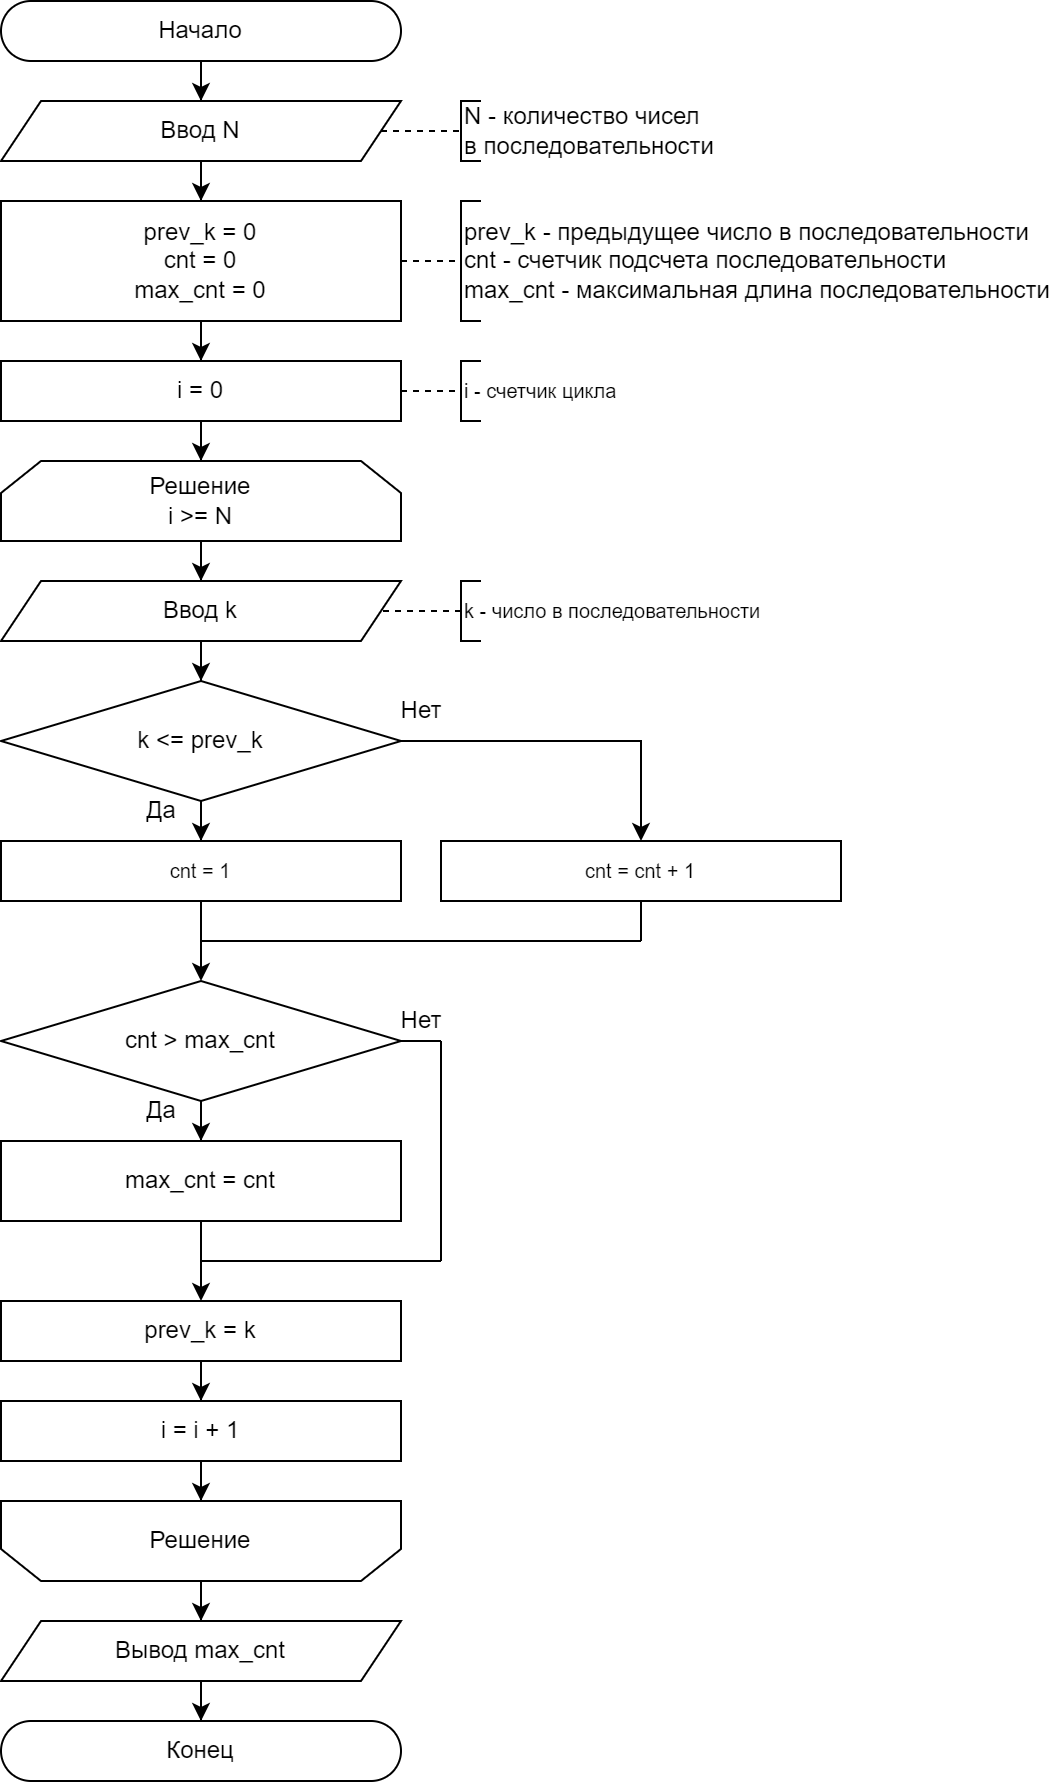
\includegraphics[width=0.6\linewidth]{schemes/t-1}
  \end{figure}
  \begin{center}
    Рисунок 1 – Схема алгоритма задания 1
  \end{center}

  \begin{lstlisting}
#include <stdio.h>
int main() {
    int N;
    scanf("%d", &N);
    int prev_k = 0;
    int cnt = 0;
    int max_cnt = 0;
    for (int i = 0; i < N; i++) {
        int k;
        scanf("%d", &k);
        if (k <= prev_k) {
            cnt = 1;
        } else {
            cnt++;
        }
        if (cnt > max_cnt) {
            max_cnt = cnt;
        }
        prev_k = k;
    }
    printf("%d", max_cnt);
    return 0;
}
  \end{lstlisting}

  \subsection*{Задание 2}
  \begin{figure}[h]
    \centering
    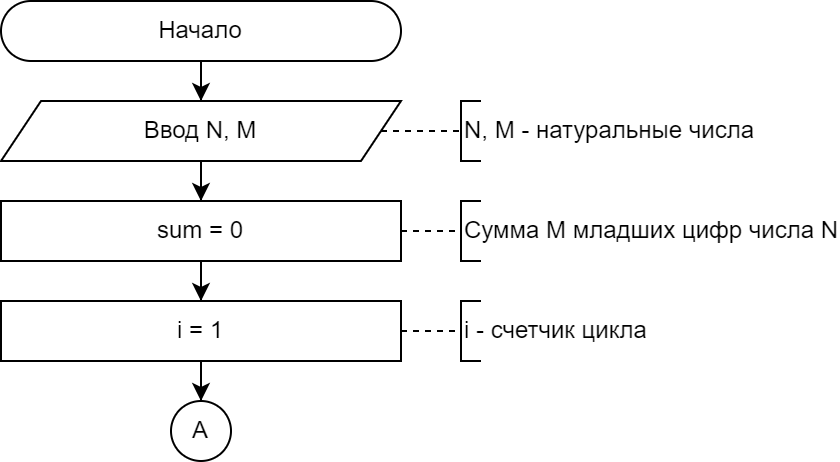
\includegraphics[width=0.6\linewidth]{schemes/t-2-1}
  \end{figure}
  \begin{center}
    Рисунок 2.1 – Схема алгоритма задания 2
  \end{center}

  \pagebreak
  \begin{figure}[h]
    \centering
    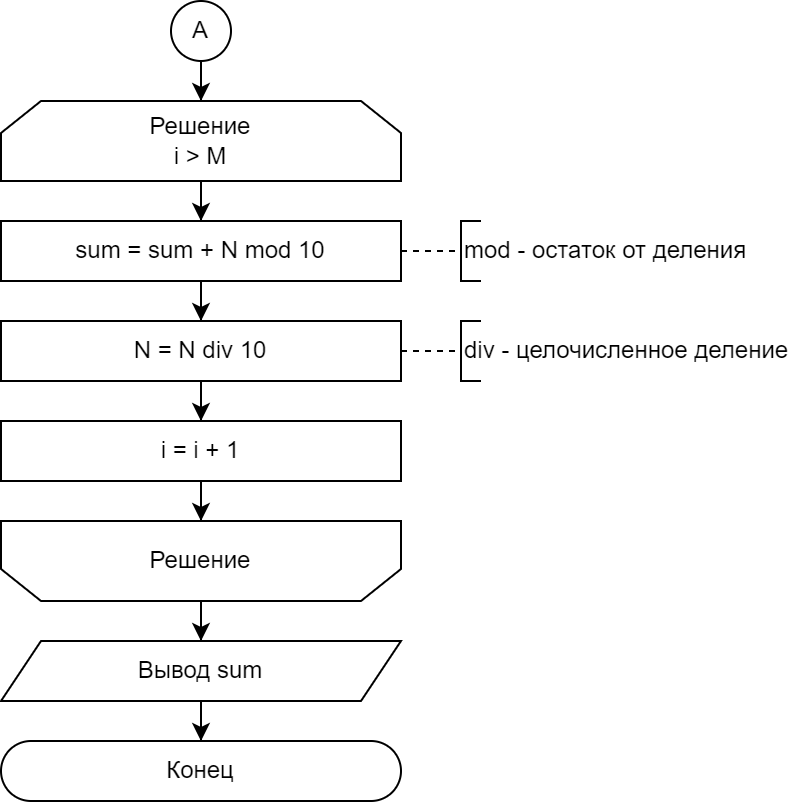
\includegraphics[width=0.6\linewidth]{schemes/t-2-2}
  \end{figure}
  \begin{center}
    Рисунок 2.2 – Продолжение схемы алгоритма задания 2
  \end{center}

  \begin{lstlisting}
program task2;
var M, sum, i:integer;
var N:longint;
begin
    readln(N);
    readln(M);
    sum := 0;
    for i := 1 to M do
    begin
        sum += N mod 10;
        N := N div 10;
    end;
    writeln(sum);
end.
  \end{lstlisting}

  \pagebreak
  \subsection*{Задание 3}
  \begin{figure}[h]
    \centering
    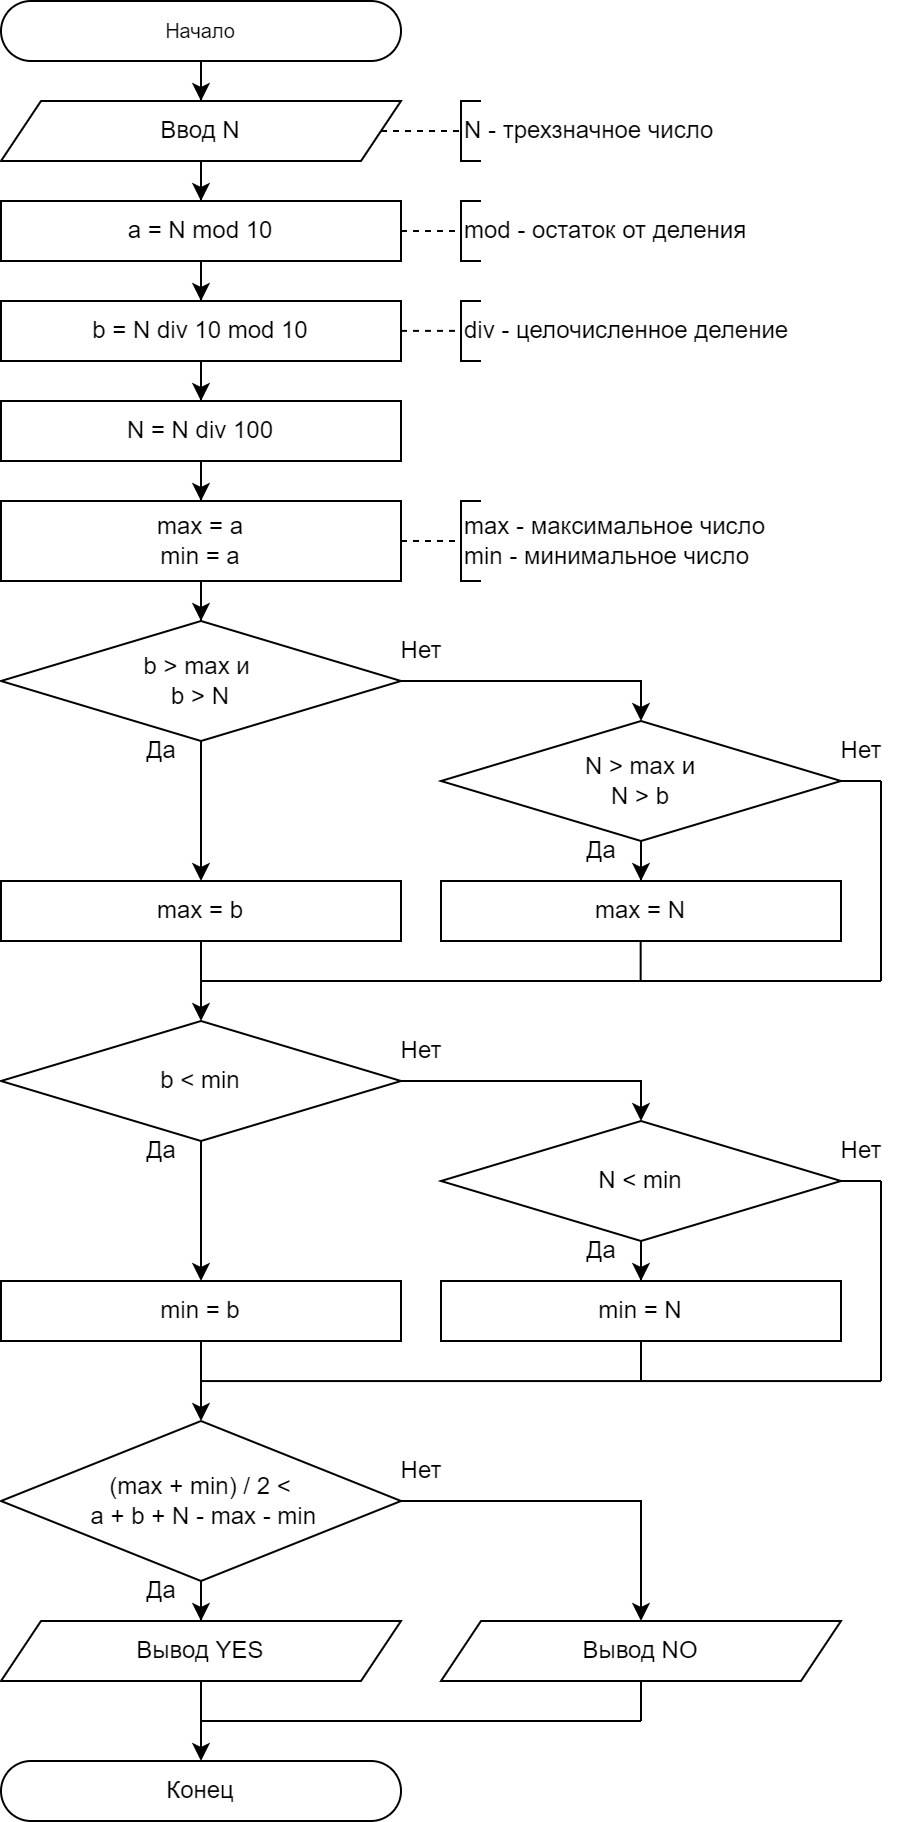
\includegraphics[width=0.58\linewidth]{schemes/t-3}
  \end{figure}
  \begin{center}
    Рисунок 3 – Схема алгоритма задания 3
  \end{center}

  \pagebreak
  \begin{lstlisting}
#include <stdio.h>
int main() {
    int N; 
    scanf("%d", &N);
    int a = N % 10;
    int b = N / 10 % 10;
    N /= 100;
    int max = a;
    int min = a;
    if (b > max && b > N) {
      max = b;
    } else if (N > max && N > b) {
      max = N;
    }
    if (b < min) {
      min = b;
    } else if (N < min) {
      min = N;
    }
    if ((max + min) / 2 < a + b + N - max - min) {
      printf("YES");
    } else {
       printf("NO");
    }
    return 0;
}
  \end{lstlisting}

  \pagebreak
  \subsection*{Задание 4}
  \begin{figure}[h]
    \centering
    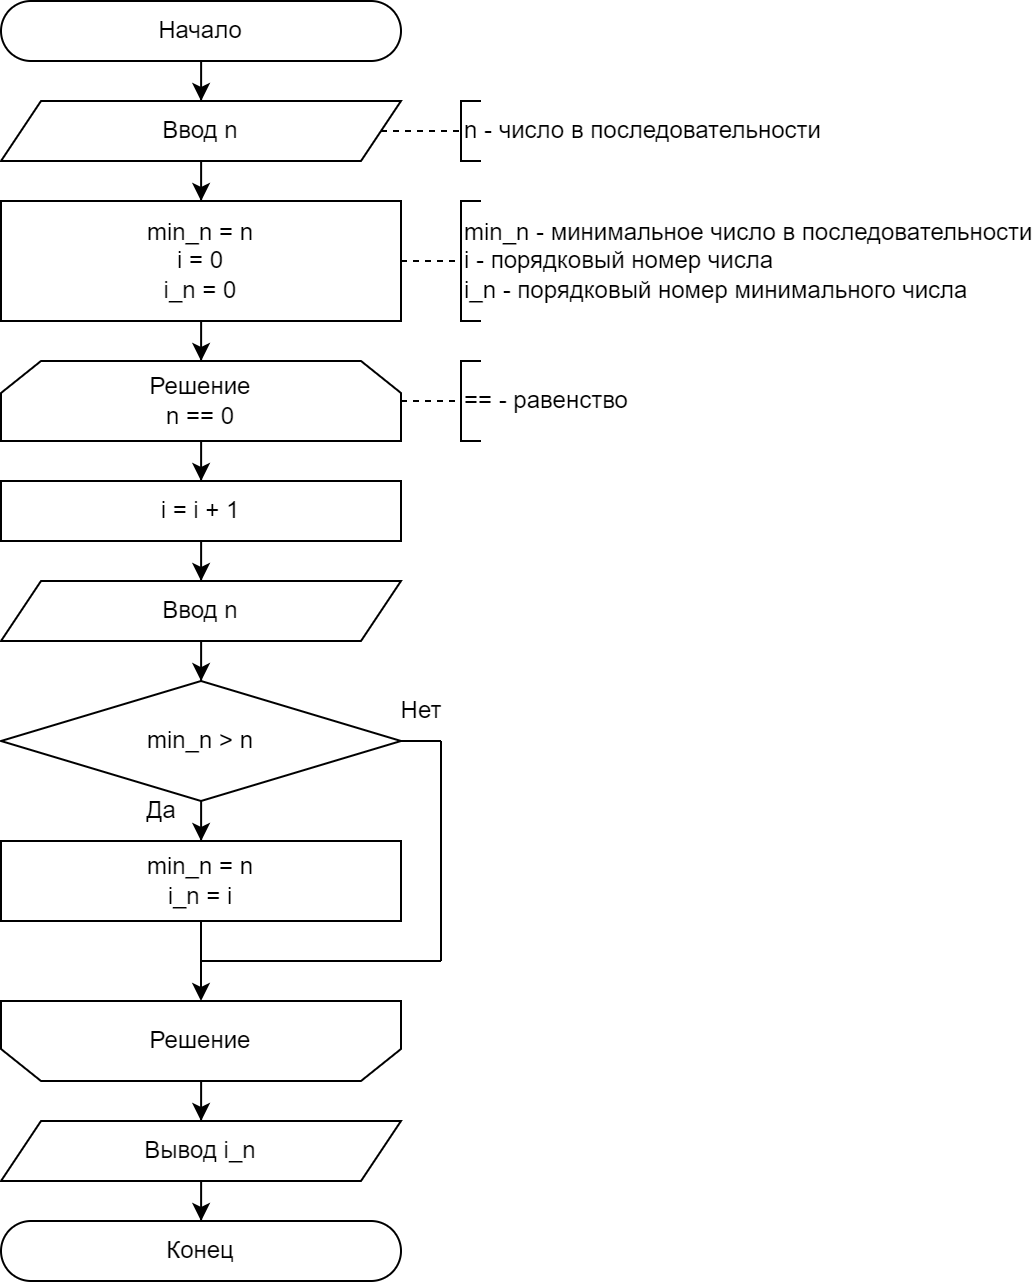
\includegraphics[width=0.6\linewidth]{schemes/t-4}
  \end{figure}
  \begin{center}
    Рисунок 4 – Схема алгоритма задания 4
  \end{center}

  \begin{lstlisting}
program task4;
var n, min_n, i, i_n:integer;
begin
read(n);
    min_n := n;
    i := 0;
    i_n := 0;
    while n <> 0 do
    begin
        i += 1;
        read(n);
        if min_n > n then
        begin
            min_n := n;
            i_n := i;
        end;
    end;
    writeln(i_n);
end.
  \end{lstlisting}

  \subsection*{Задание 5}
  \begin{figure}[h]
    \centering
    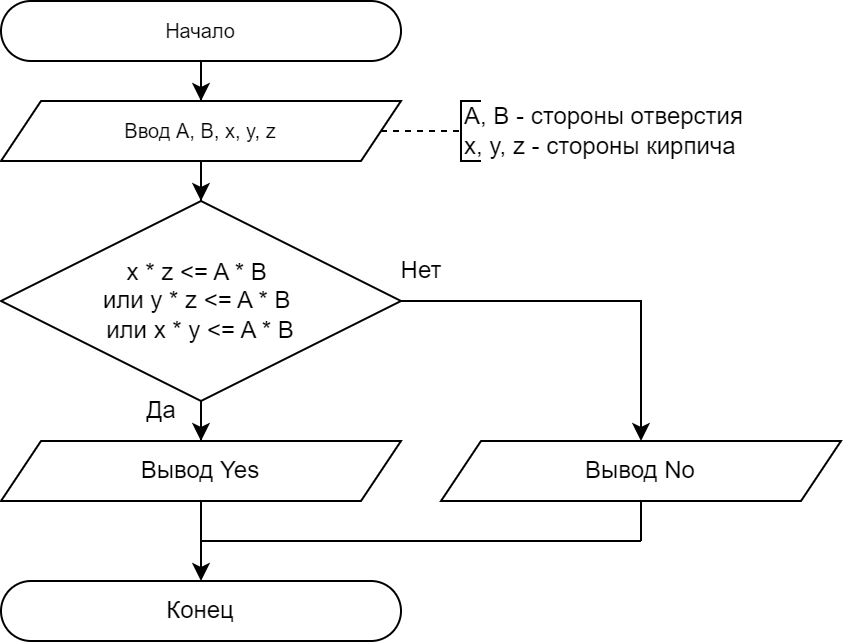
\includegraphics[width=0.6\linewidth]{schemes/t-5}
  \end{figure}
  \begin{center}
    Рисунок 5 – Схема алгоритма задания 5
  \end{center}

  \begin{lstlisting}
#include <stdio.h>
int main() {
    int A;
    int B;
    int x;
    int y;
    int z;
    scanf("%d %d %d %d %d", &A, &B, &x, &y, &z);
    if (x * z <= A * B 
        || y * z <= A * B 
        || x * y <= A * B) {
        printf("Yes");
    } else {
        printf("No");
    }
    return 0;
}
  \end{lstlisting}

  \subsection*{Задание 6}
  \begin{figure}[h]
    \centering
    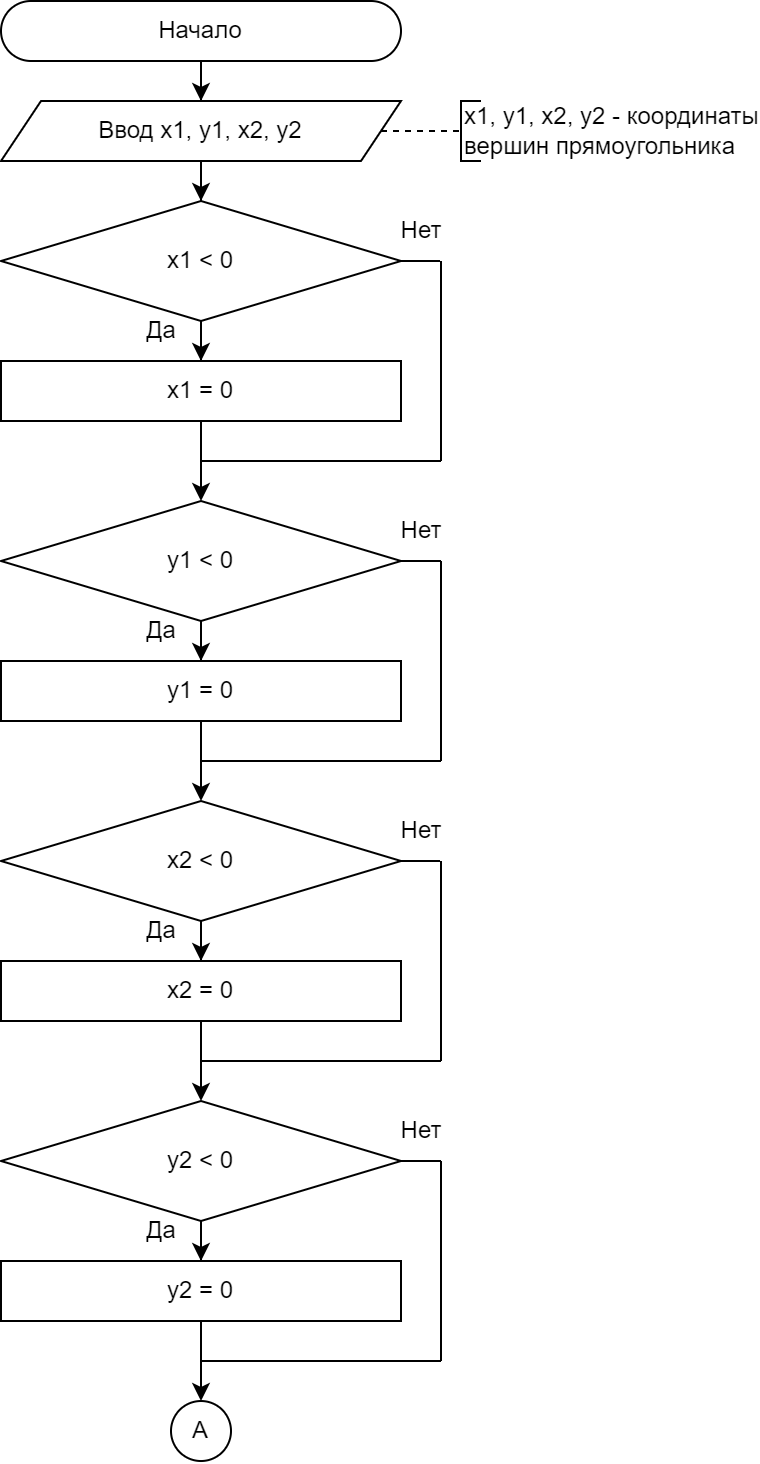
\includegraphics[width=0.5\linewidth]{schemes/t-6-1}
  \end{figure}
  \begin{center}
    Рисунок 6.1 – Схема алгоритма задания 6
  \end{center}

  \pagebreak
  \begin{figure}[h]
    \centering
    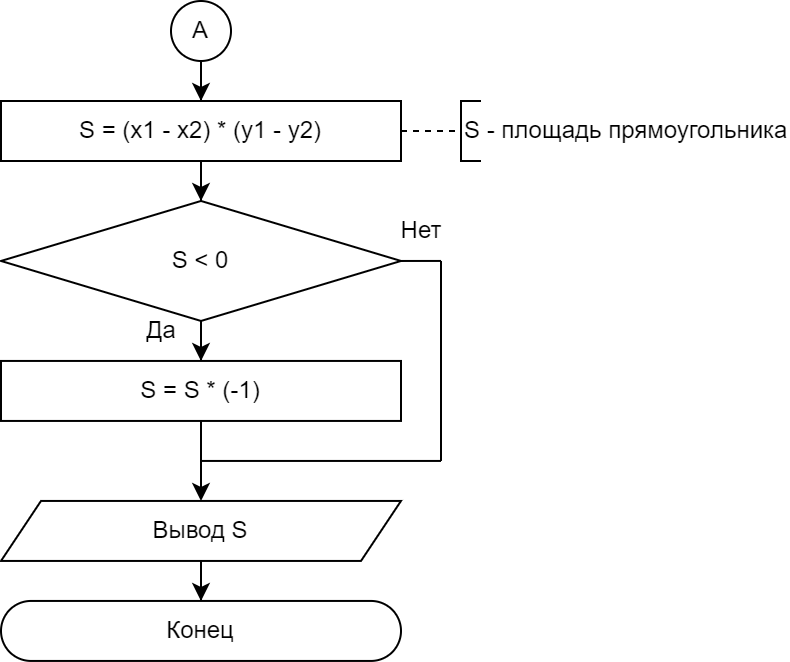
\includegraphics[width=0.6\linewidth]{schemes/t-6-2}
  \end{figure}
  \begin{center}
    Рисунок 6.2 – Продолжение схемы алгоритма задания 6
  \end{center}

  \begin{lstlisting}
program task6;
var x1, y1, x2, y2, S:int64;
begin
    readln(x1, y1, x2, y2);
    if x1 < 0 then
        x1 := 0;
    if y1 < 0 then
        y1 := 0;
    if x2 < 0 then
        x2 := 0;
    if y2 < 0 then
        y2 := 0;
    S := (x1 - x2) * (y1 - y2);
    if S < 0 then
        S *= -1;
    writeln(S);
end.
  \end{lstlisting}

  \pagebreak
  \subsection*{Задание 7}
  \begin{figure}[h]
    \centering
    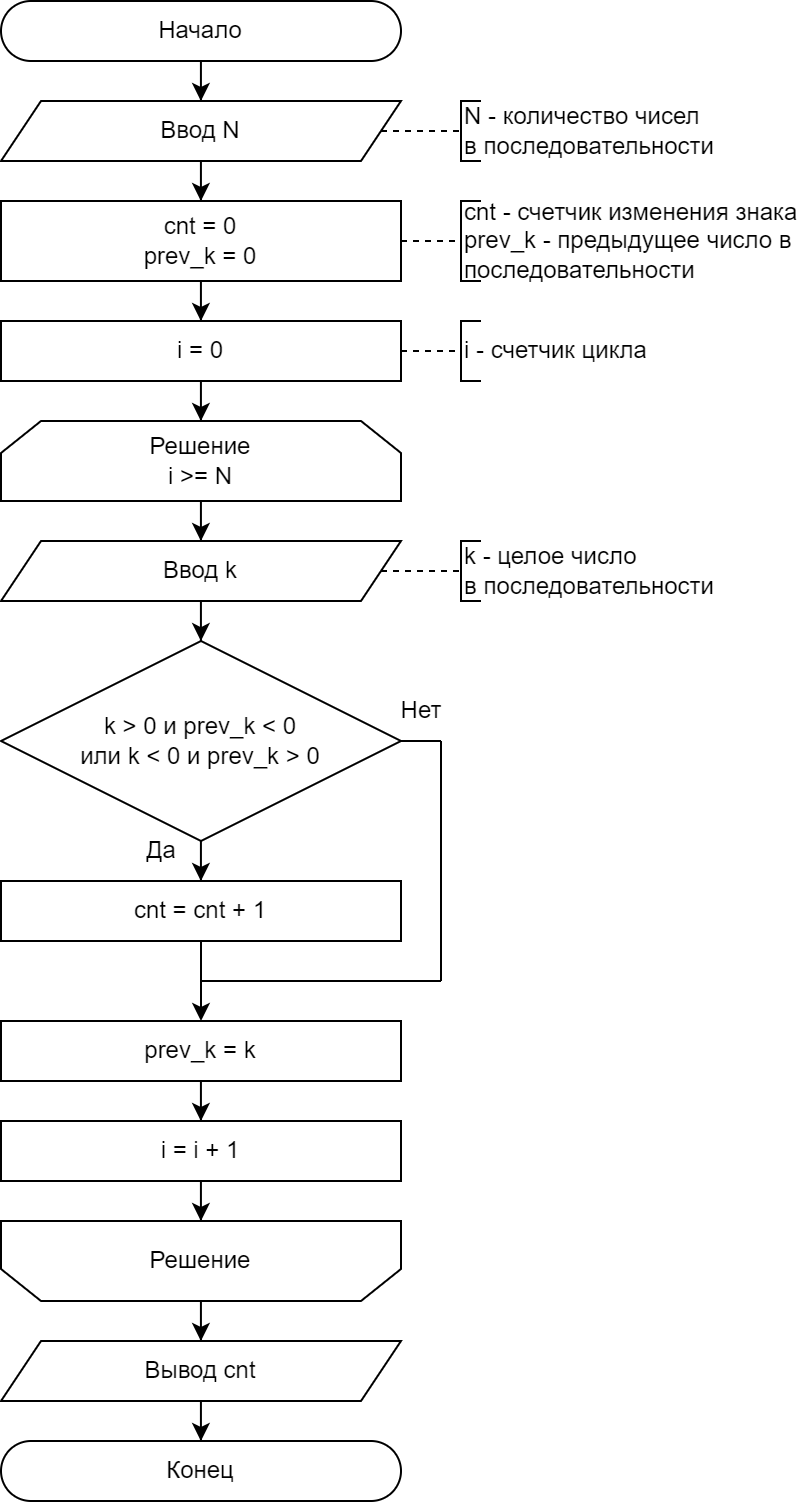
\includegraphics[width=0.6\linewidth]{schemes/t-7}
  \end{figure}
  \begin{center}
    Рисунок 7 – Схема алгоритма задания 7
  \end{center}

  \begin{lstlisting}
#include <stdio.h>
int main() {
    int N;
    scanf("%d", &N);	
    int cnt = 0;
    int prev_k = 0;
    for (int i = 0; i < N; i++) {
        int k;
        scanf("%d", &k);
        if (k > 0 && prev_k < 0 
            || k < 0 && prev_k > 0) {
            cnt++;
        }
        prev_k = k;
    }
    printf("%d", cnt);
    return 0;
}
  \end{lstlisting}

  \subsection*{Задание 8}
  \begin{figure}[h]
    \centering
    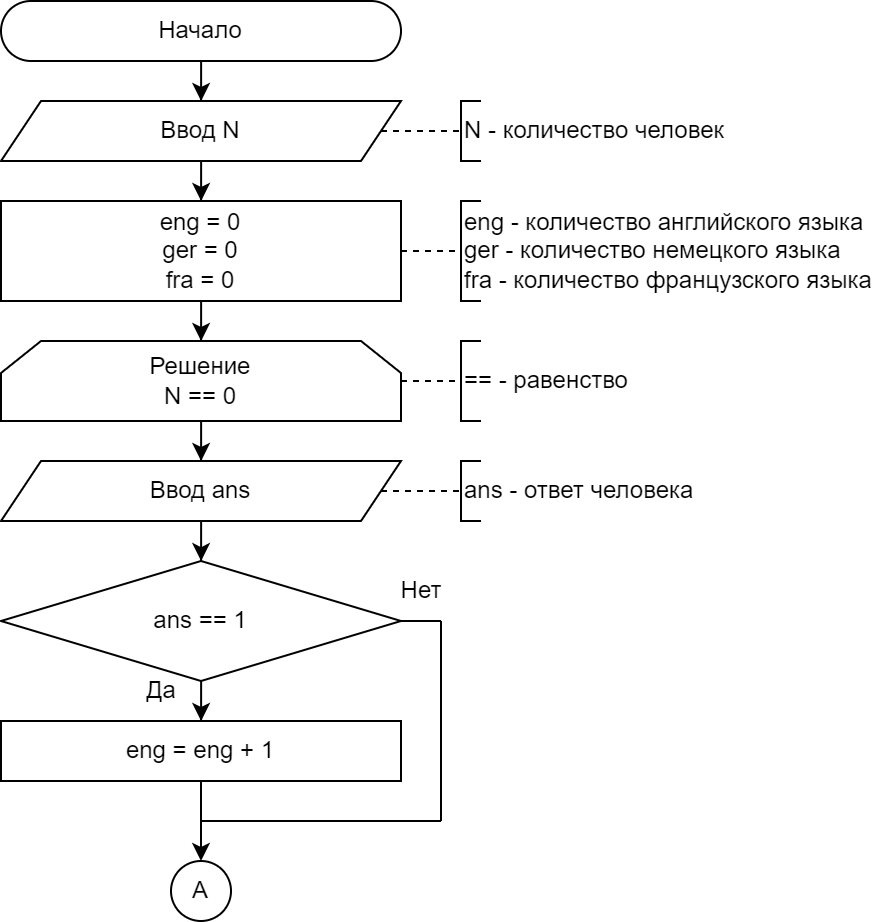
\includegraphics[width=0.6\linewidth]{schemes/t-8-1}
  \end{figure}
  \begin{center}
    Рисунок 8.1 – Схема алгоритма задания 8
  \end{center}

  \pagebreak
  \begin{figure}[h]
  \centering
  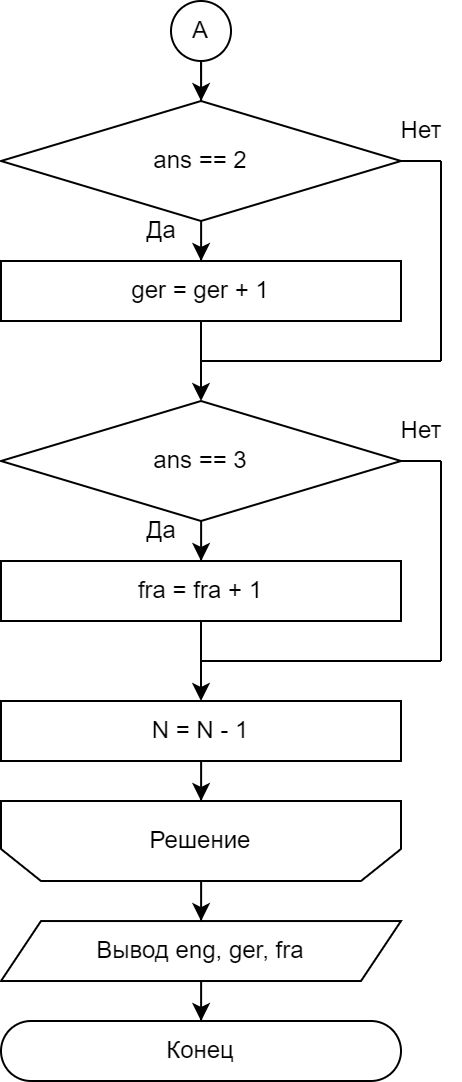
\includegraphics[width=0.35\linewidth]{schemes/t-8-2}
  \end{figure}
  \begin{center}
    Рисунок 8.2 – Продолжение схемы алгоритма задания 8
  \end{center}

  \begin{lstlisting}
program task8;
var N, i, ans, eng, ger, fra:integer;
begin
    readln(N);
    eng := 0;
    ger := 0;
    fra := 0;
    while N <> 0 do
    begin
        readln(ans);
        if ans = 1 then
            eng += 1;
        if ans = 2 then
            ger += 1;
        if ans = 3 then
            fra += 1;
        N -= 1
    end;
    writeln(eng);
    writeln(ger);
    writeln(fra);
end.
  \end{lstlisting}

  \subsection*{Задание 9}
  \begin{figure}[h]
    \centering
    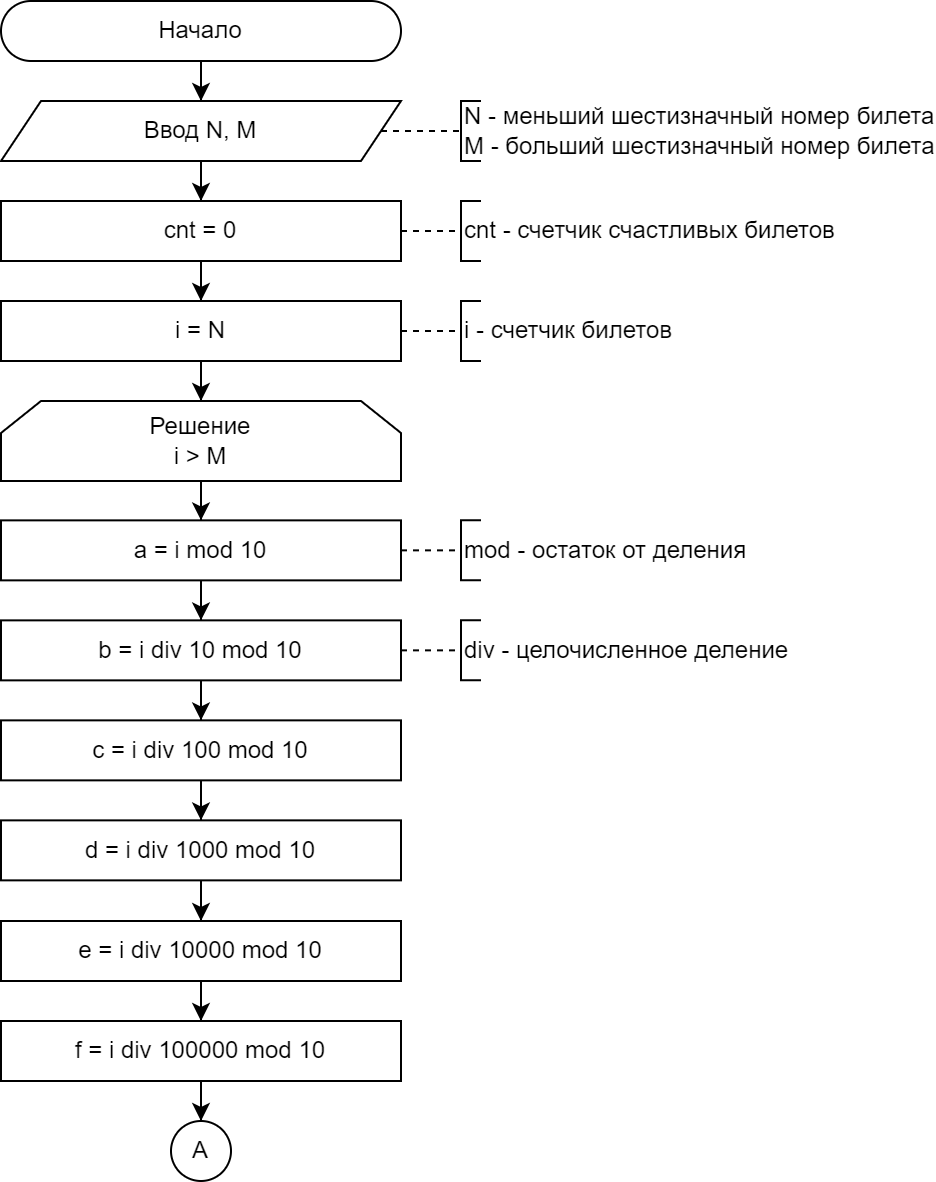
\includegraphics[width=0.6\linewidth]{schemes/t-9-1}
  \end{figure}
  \begin{center}
    Рисунок 9.1 – Схема алгоритма задания 9
  \end{center}

  \pagebreak
  \begin{figure}[h]
    \centering
    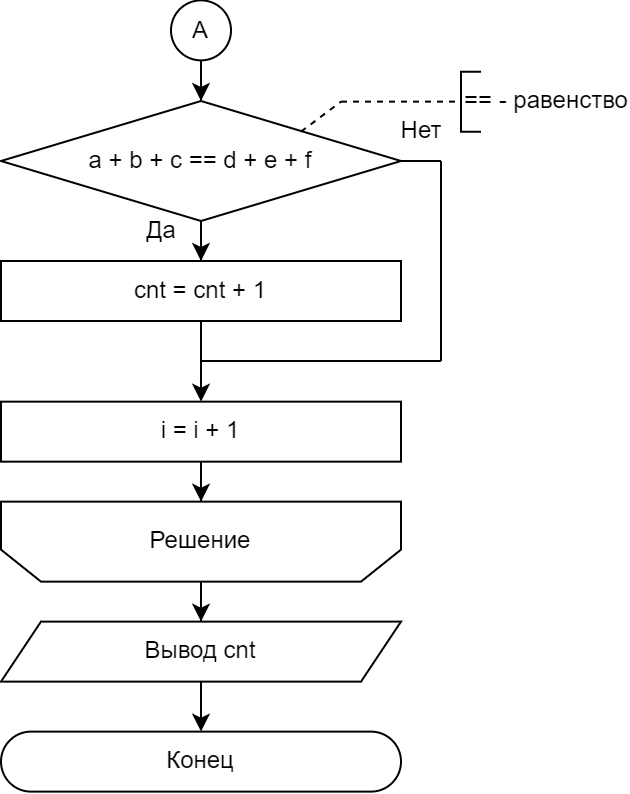
\includegraphics[width=0.35\linewidth]{schemes/t-9-2}
  \end{figure}
  \begin{center}
    Рисунок 9.2 – Продолжение схемы алгоритма задания 9
  \end{center}

  \begin{lstlisting}
#include <stdio.h>
int main() {
    int N;
    int M;
    scanf("%d %d", &N, &M);
    int cnt = 0;
    for (int i = N; i <= M; i++) {
        int a = i % 10;
        int b = i / 10 % 10;
        int c = i / 100 % 10;
        int d = i / 1000 % 10;
        int e = i / 10000 % 10;
        int f = i / 100000 % 10;

        if ((a + b + c) == (d + e + f)) {
            cnt++;
        }
    }
    printf("%d", cnt);
    return 0;
}
  \end{lstlisting}

  \subsection*{Задание 10}
  \begin{figure}[h]
    \centering
    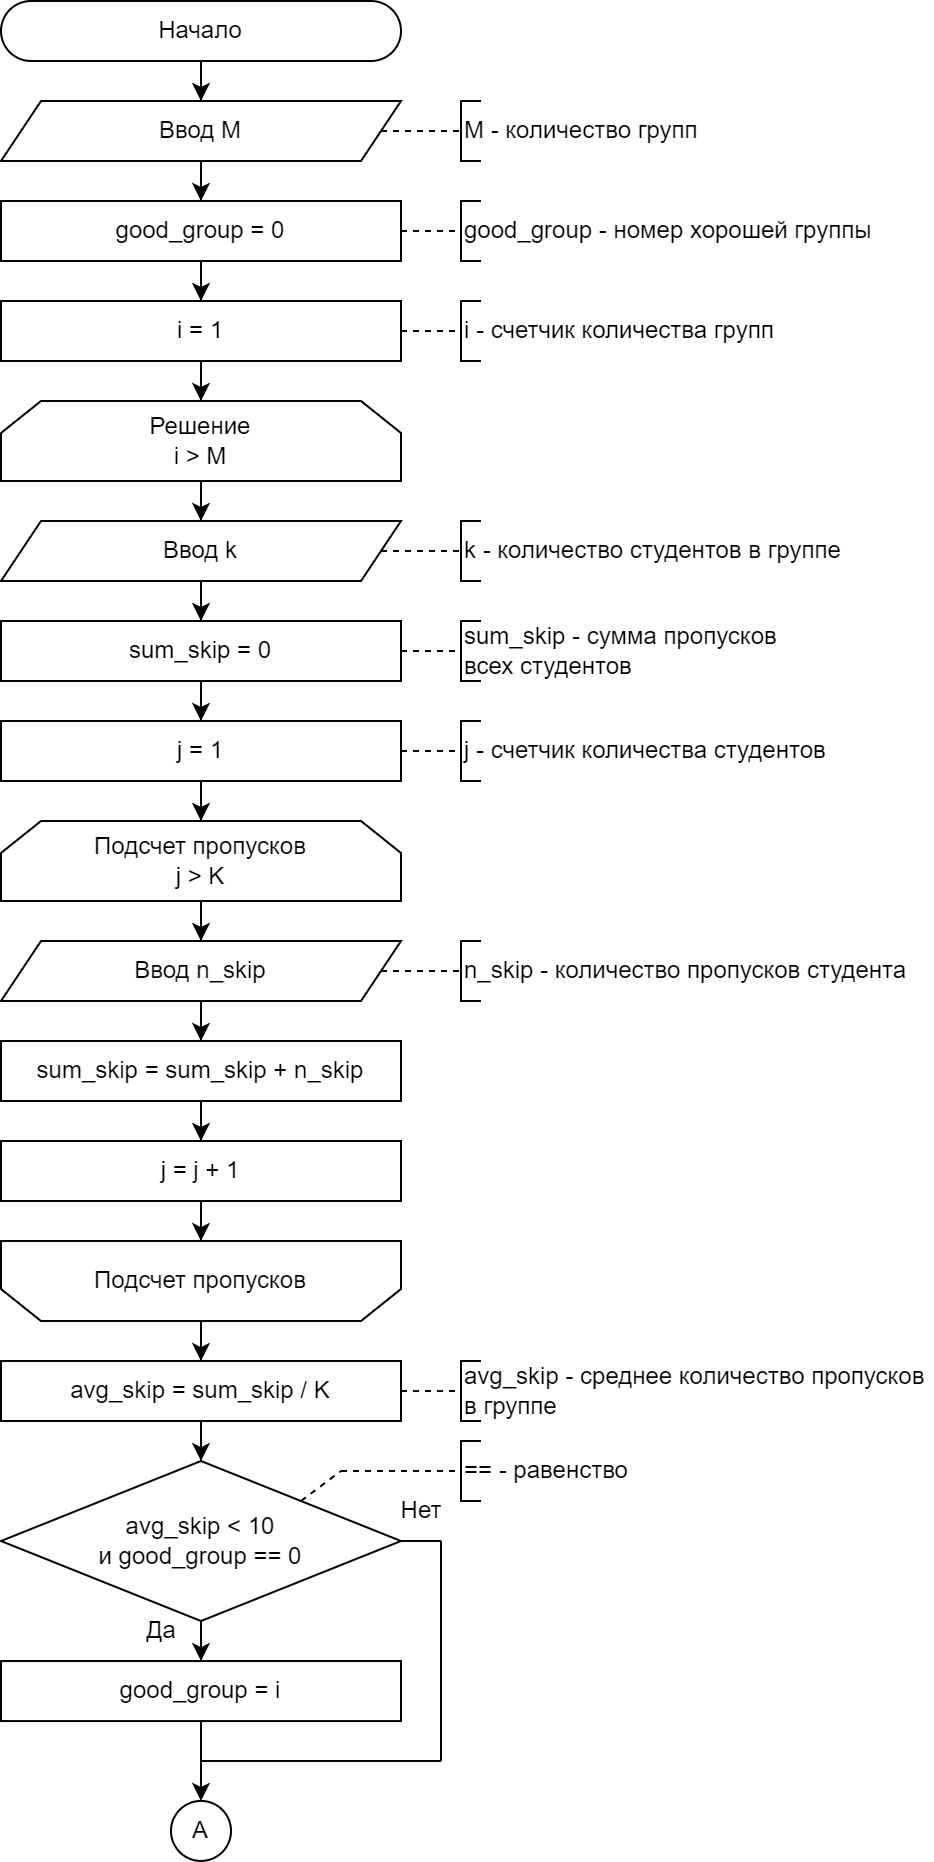
\includegraphics[width=0.6\linewidth]{schemes/t-10-1}
  \end{figure}
  \begin{center}
    Рисунок 10.1 – Схема алгоритма задания 10
  \end{center}

  \pagebreak
  \begin{figure}[h]
    \centering
    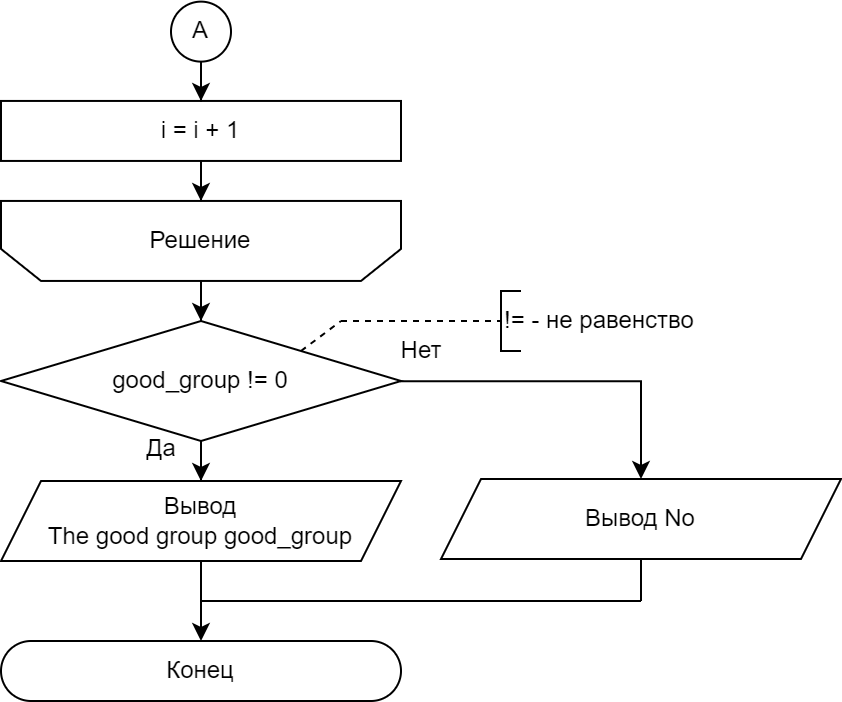
\includegraphics[width=0.55\linewidth]{schemes/t-10-2}
  \end{figure}
  \begin{center}
    Рисунок 10.2 – Продолжение схемы алгоритма задания 10
  \end{center}

  \begin{lstlisting}
program task10;
var M, K, i, j, good_group, sum_skip, n_skip:integer;
var avg_skip:real;
begin
    readln(M);
    good_group := 0;
    for i := 1 to M do
    begin
        read(K);
        sum_skip := 0;
        for j := 1 to K do
        begin
            read(n_skip);
            sum_skip += n_skip;
        end;
        avg_skip := sum_skip / K;
        if (avg_skip < 10) and (good_group = 0) then
            good_group := i;
    end;
    if (good_group <> 0) then
        writeln('The good group ', good_group)
    else
        writeln('No');
end.
  \end{lstlisting}

  \subsection*{Задание 11}
  \begin{figure}[h]
    \centering
    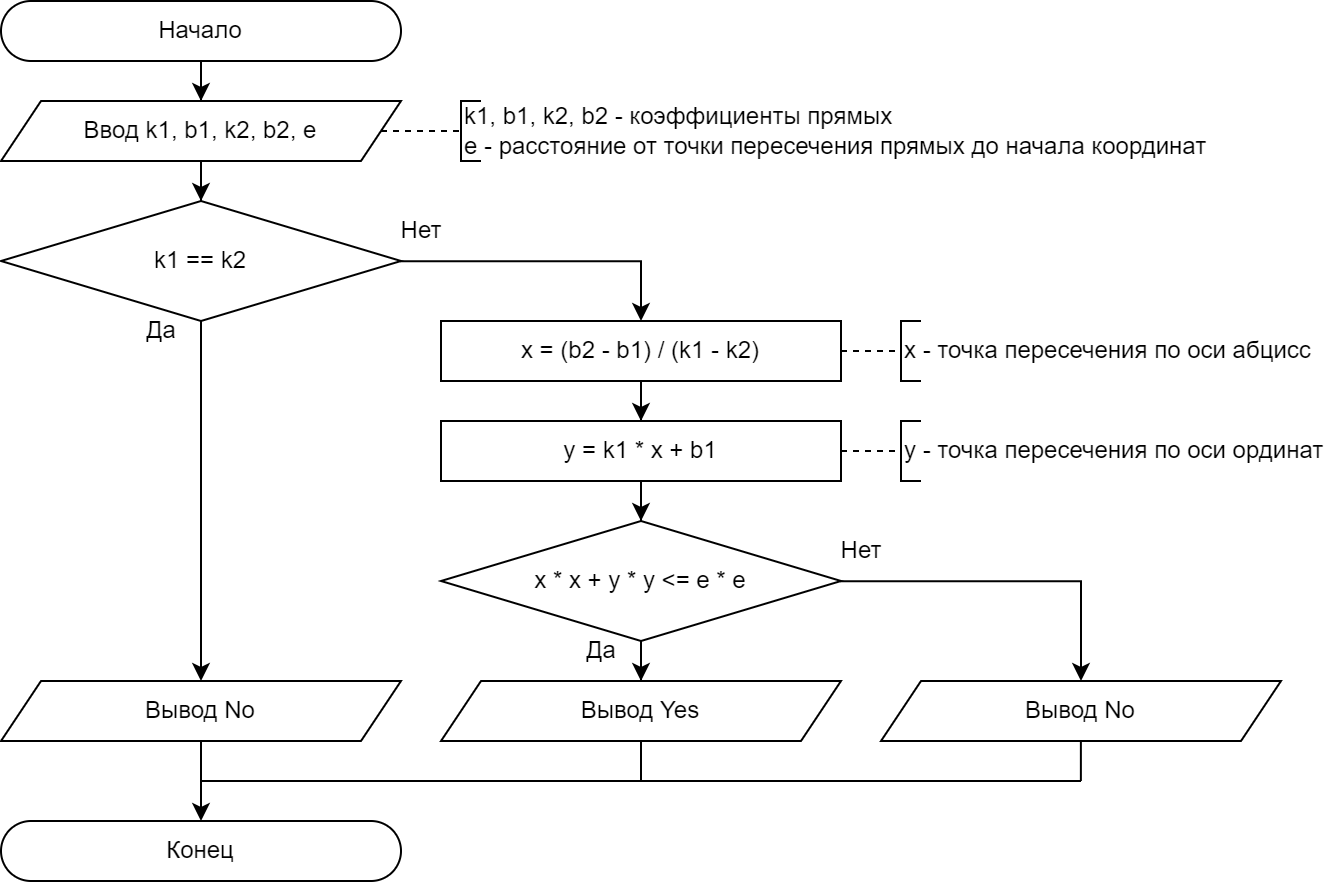
\includegraphics[width=0.6\linewidth]{schemes/t-11}
  \end{figure}
  \begin{center}
    Рисунок 11 – Схема алгоритма задания 11
  \end{center}

  \begin{lstlisting}
#include <stdio.h>
int main() {
    float k1;
    float b1;
    float k2;
    float b2;
    float e;
    scanf("%f %f %f %f %f", &k1, &b1, &k2, &b2, &e);
    if (k1 == k2) {
        printf("No");
    } else {
        float x = (b2 - b1) / (k1 - k2);
        float y = k1 * x + b1;
        if (x * x + y * y <= e * e) {
            printf("Yes");
        } else {
            printf("No");
        }
    }
    return 0;
}
  \end{lstlisting}

  \subsection*{Задание 12}
  \begin{figure}[h]
    \centering
    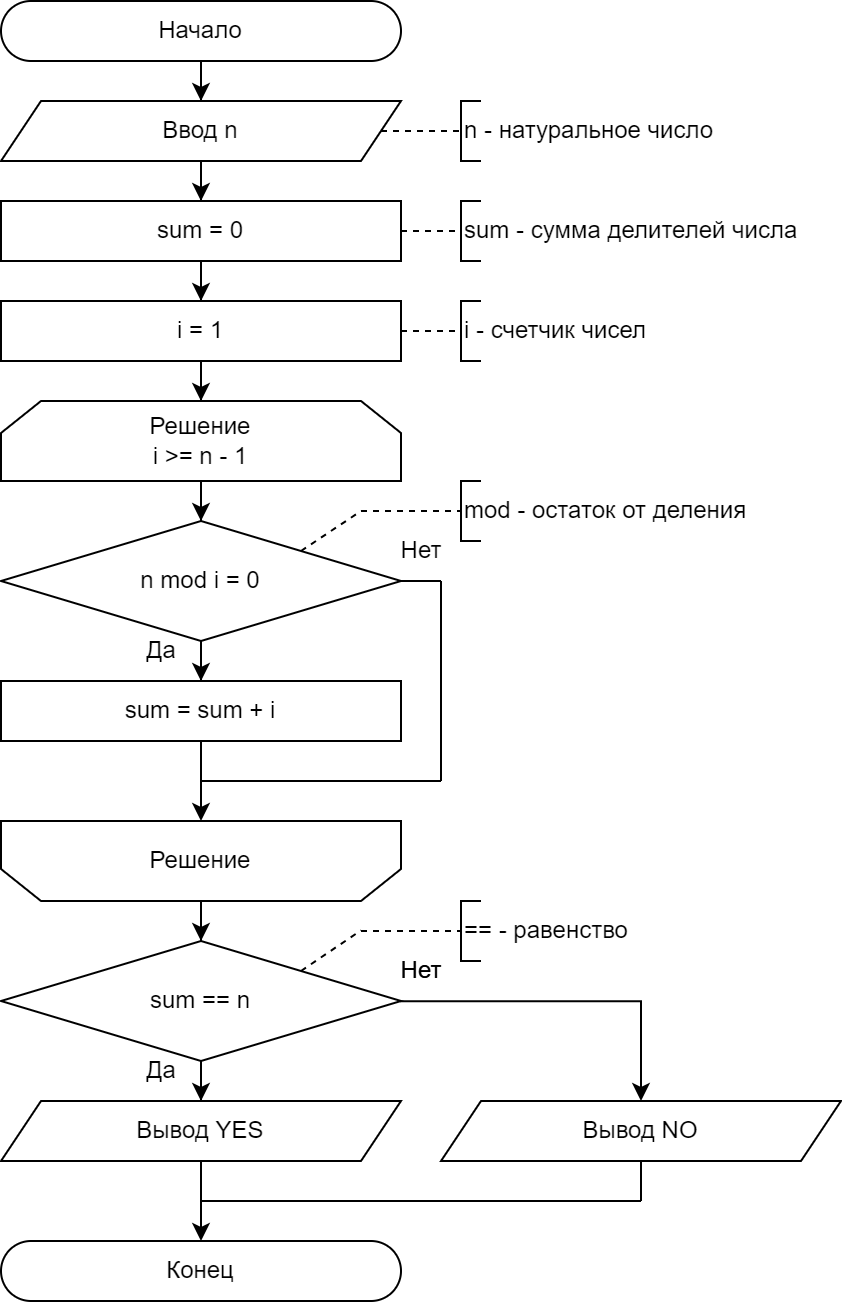
\includegraphics[width=0.6\linewidth]{schemes/t-12}
  \end{figure}
  \begin{center}
    Рисунок 12 – Схема алгоритма задания 12
  \end{center}

  \begin{lstlisting}
program task12;
var n, i, sum:integer;
begin
    readln(n);
    sum := 0;
    for i := 1 to n - 1 do
    begin
        if n mod i = 0 then
            sum += i;
    end;
    if sum = n then
        writeln('YES')
    else
        writeln('NO');
end.
  \end{lstlisting}

  \section*{Вывод}
  В ходе выполнения лабораторной работы были решены задачи, которые позволили закрепить и освоить на практике знания о использовании арифметических операций, условных конструкций, циклов, а также корректной типизации данных.

\end{document}